于是
$$
    \diag(\vb) = 
     \begin{tikzpicture}[baseline=\baseline]
    \tikzset{tensor/.style = {minimum size = 0.5cm,shape = circle,thick,draw=black,inner sep = 0pt}, edge/.style   = {thick,line width=.4mm},every loop/.style={}}
    \def\y{0}
    \def\x{0}
    \draw  node[fill = black,circle,inner sep=0pt,minimum size=4pt] (m) at (\x,\y) {};
    \node[tensor,fill=blue!20!red!40!white] (v) at (\x,\y-0.85){\scalebox{0.85}{$\vb$}};
    \draw[edge] (m) -- (\x-0.6,0);
    \draw[edge] (m) -- (\x+0.6,0);
    \draw[edge] (m) -- (\x,\y-0.6); 
    \node[draw=none] at (\x+1,\y) {\scalebox{1}{\textcolor{black}{$=$}}};
    \node[tensor,fill=blue!20!red!40!white] (v) at (\x+2.5,\y){\scalebox{0.85}{}};
    \draw[edge] (v) -- (\x+3.5,\y);
    \draw[edge] (v) -- (\x+1.5,\y);
  \draw[edge=0.5] (v.south west) -- (v.north east);
\end{tikzpicture} 
~~\text{and}~~
\diag(\Ab) =\hspace{-0.7cm}
\begin{tikzpicture}[baseline=\baseline]
    \tikzset{tensor/.style = {minimum size = 0.5cm,shape = circle,thick,draw=black,inner sep = 0pt}, edge/.style = {thick,line width=.4mm},every loop/.style={}}
    \def\y{0}
    \def\x{0}
    \node[tensor,fill=red!50!white] (A) at (\x,\y+0.2){\scalebox{0.85}{$\Ab$}};
    \draw[edge] (A) to [out=-20,in=-160, distance=1.35cm] (A);
    \draw  node[fill = black,circle,inner sep=0pt,minimum size=4pt] (m) at (\x,\y-0.25) {};
    \draw[edge] (m) -- (\x,\y-0.65);
    \end{tikzpicture},
$$
其中
$
\begin{tikzpicture}[baseline=\baseline]
    \tikzset{tensor/.style = {minimum size = 0.5cm,shape = circle,thick,draw=black,inner sep = 0pt}, edge/.style = {thick,line width=.4mm},every loop/.style={}}
    \def\y{0}
    \def\x{0}
    \node[tensor,fill=blue!20!red!40!white] (v) at (\x+2.5,\y){\scalebox{0.85}{}};
    \draw[edge] (v) -- (\x+3.5,\y);
    \draw[edge] (v) -- (\x+1.5,\y);
  \draw[edge=0.5] (v.south west) -- (v.north east);
\end{tikzpicture} 
$ 
表示一个对角矩阵。
\begin{proof}
第一条：对任意 $i,j\in [n]$，有
\begin{align*}
    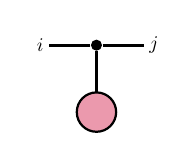
\begin{tikzpicture}[baseline=-15]
    \tikzset{tensor/.style = {minimum size = 0.5cm,shape = circle,thick,draw=black,inner sep = 0pt}, edge/.style   = {thick,line width=.4mm},every loop/.style={}}
    \def\y{0}
    \def\x{0}
    \draw  node[fill = black,circle,inner sep=0pt,minimum size=4pt] (m) at (\x,\y) {};
   \node[tensor,fill=blue!20!red!40!white] (v) at (\x,\y-0.85){\scalebox{0.85}{$\vb$}};
    \draw[edge] (m) -- (\x-0.6,0) node [very near end,left] {\scalebox{0.7}{\indcolor{$i$}}};
    \draw[edge] (m) -- (\x+0.6,0)node [very near end,right] {\scalebox{0.7}{\indcolor{$j$}}};;
    \draw[edge] (m) -- (\x,\y-0.6);
 \end{tikzpicture}
&=
 \sum_{k}
\left(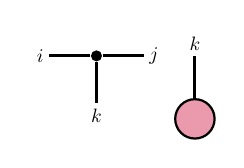
\begin{tikzpicture}[baseline=-15]
    \tikzset{tensor/.style = {minimum size = 0.5cm,shape = circle,thick,draw=black,inner sep = 0pt}, edge/.style   = {thick,line width=.4mm},every loop/.style={}}
    \def\y{0}
    \def\x{0}
    \draw  node[fill = black,circle,inner sep=0pt,minimum size=4pt] (m) at (\x,\y) {};
    \draw[edge] (m) -- (\x-0.6,0)node [very near end, left] {\scalebox{0.7}{\indcolor{$i$}}};;
    \draw[edge] (m) -- (\x+0.6,0)node [very near end, right] {\scalebox{0.7}{\indcolor{$j$}}};
    \draw[edge] (m) -- (\x,\y-0.6)node [very near end, below]{\scalebox{0.7}{\indcolor{$k$}}};  \node[tensor,fill=blue!20!red!40!white] (v) at (\x+1.25,\y-0.8){\scalebox{0.85}{$\vb$}};
    \draw[edge] (v) -- (\x+1.25,0)node [very near end, above] {\scalebox{0.7}{\indcolor{$k$}}};;
 \end{tikzpicture}\right)\\
&= 
\sum_{k}\delta_{ijk}\vb_k = 
\delta_{ij}\vb_i
= 
\begin{cases}
\vb_i & \text{ if } i=j\\
0 &\text{ otherwise}
\end{cases}
= \text{diag}(\vb)_{ij}.
\end{align*}
第二条：对任意 $i\in [n]$，有
\begin{align*}
    \begin{tikzpicture}[baseline=\baseline]
    \tikzset{tensor/.style = {minimum size = 0.5cm,shape = circle,thick,draw=black,inner sep = 0pt}, edge/.style = {thick,line width=.4mm},every loop/.style={}}
    \def\y{0}
    \def\x{0}
    \node[tensor,fill=red!50!white] (A) at (\x,\y+0.2){\scalebox{0.85}{$\Ab$}};
    \draw[edge] (A) to [out=-20,in=-160, distance=1.35cm] (A);
    \draw  node[fill = black,circle,inner sep=0pt,minimum size=4pt] (m) at (\x,\y-0.25) {};
    \draw[edge] (m) -- (\x,\y-0.65)node [very near end, below] {\scalebox{0.7}{\indcolor{$i$}}};
\end{tikzpicture}\hspace{-0.7cm}
=
\sum_{j,k}\left(
\begin{tikzpicture}[baseline=\baseline]
    \tikzset{tensor/.style = {minimum size = 0.5cm,shape = circle,thick,draw=black,inner sep = 0pt}, edge/.style = {thick,line width=.4mm},every loop/.style={}}
    \def\y{0}
    \def\x{0}
    \node[tensor,fill=red!50!white] (A) at (\x,\y+0.4){\scalebox{0.85}{$\Ab$}};
    \draw  node[fill = black,circle,inner sep=0pt,minimum size=4pt] (m) at (\x,\y-0.25) {};
    \draw[edge] (m) -- (\x-0.7,\y-0.25)node [very near end,left] {\scalebox{0.7}{\indcolor{$k$}}};
    \draw[edge] (m) -- (\x+0.7,\y-0.25)node [very near end,right] {\scalebox{0.7}{\indcolor{$j$}}};
    \draw[edge] (m) -- (\x,\y-0.75)node [very near end, below] {\scalebox{0.7}{\indcolor{$i$}}};
    \draw[edge] (A) --(\x+0.7,\y+0.4)node [very near end,right] {\scalebox{0.7}{\indcolor{$j$}}};
    \draw[edge] (A) --(\x-0.7,\y+0.4)node [very near end,left] {\scalebox{0.7}{\indcolor{$k$}}};
    \end{tikzpicture}\right)
=
\sum_{j,k}\delta_{ijk}\Ab_{kj}
=
\Ab_{ii} = \diag(\Ab)
_{i}.
\end{align*}
\end{proof}
\item\label{prop:diag}
由此不难验证 $\diag(\vb)\diag(\ub)$ =
    \begin{tikzpicture}[baseline=\baseline]
    \tikzset{tensor/.style = {minimum size = 0.5cm,shape = circle,thick,draw=black,inner sep = 0pt}, edge/.style   = {thick,line width=.4mm},every loop/.style={}}
    \def\y{0}
    \def\x{0}
    \draw  node[fill = black,circle,inner sep=0pt,minimum size=4pt] (m) at (\x,\y) {};
    \node[tensor,fill=blue!20!red!40!white] (v) at (\x,\y-0.85){\scalebox{0.85}{$\vb$}};
    \draw[edge] (m) -- (\x-0.6,0);
    \draw[edge] (m) -- (\x,\y-0.6); 
    \draw  node[fill = black,circle,inner sep=0pt,minimum size=4pt] (m1) at (\x+1,\y) {};
    \node[tensor,fill=red!20!blue!40!white] (u) at (\x+1,\y-0.85){\scalebox{0.85}{$\ub$}};
    \draw[edge] (m1) -- (m);
    \draw[edge] (m1) -- (\x+1.6,0);
    \draw[edge] (m1) -- (\x+1,\y-0.6); 
\end{tikzpicture}.
\end{enumerate}
\end{proposition}

